% !TEX root = thesis.tex

\chapter{Introduction}
\label{ch:introduction}

The Dark Energy plus Cold Dark Matter (\lcdm{}) cosmological model is the current ``standard model" which satisfactorily reproduces the present-day observations of the large scale structure of the Universe, of the Cosmic Microwave Background (CMB) and of supernovae indicating an accelerating expansion of the Universe \citep{Riess1998}.
According to \lcdm{}, the Universe was formed $13.8$~Gyr ago, through the so called Big Bang, when the Universe was a hot plasma.
After a phase of sudden expansion, the consequent cooling allowed the radiation to decouple from the ordinary matter.
The last radiation scattered before the Universe became transparent is called the Cosmic Microwave Background and it is observable now in the microwave range as an uniformly distributed radiation of a black body of $2.7$~K.
Since black body spectra are produced by opaque objects CMB brings the information that the early Universe was opaque \citep{Ryden2003}.

However, at the beginning of the XX century, various measurements found that the amount of visible (baryonic) matter was not enough to justify observations of galaxy motion and their rotation.
\citet{Zwicky1933} first recognized the discrepancy and the missing matter by observing the rotation velocity of the galaxies in the outskirts of the Coma cluster \citep{Zwicky1937}.
He therefore hypothesized the existence of dark matter, a kind of matter which does not interact with the electromagnetic forces but only with gravity.
%Later observations confirmed that the missing mass could be accounted for from the rotation curves from galaxies %TODO(Babcock, 1939; Rubin & Ford, 1970; Bosma, 1978; Rubin et al., 1980).
All these observations showed that in the Universe, the amount of dark matter is around five to six times more than baryonic matter.
Another observational fact coming from supernovae, is the accelerating expansion of the Universe.
The current accepted model is the presence of an large scale unknown form of energy, called Dark Energy (or $\Lambda$), which constitutes around 68\% of al the mass-energy content of the Universe.
The \lcdm{} model also assumes that the dark matter is ``cold", \ie{} it has negligible thermal velocity and does not suppress structure formation on any scale relevant for galaxy formation \citep{Bullock2017}.
Baryonic and dark matter gravitationally collapsing slowly formed filaments along which gas could become dense enough to create self-supporting gravitational systems cradle of stars: the first galaxies.
These filaments have been observed in large surveys like the Sloan Digital Sky Survey (SDSS). % TODO figure here?

The study of galaxies has seen its development only very recently.
Less than one century ago, current recognized galaxies were thought to be small luminous clouds (and thus called \emph{nebulae}) belonging to our Galaxy, the Milky Way, the only known Galaxy.
In 1923 Edwin Hubble, measuring the distance of the \emph{nebulae} by observing their variable stars Cepheids, from the observatory of Mount Wilson in California, realized they were systems far away from the Galaxy \citep{Hubble1929}.
His observations have completely changed the view of the Universe.
The scientific research on galaxies took off from Hubble's works and even the morphological classification of galaxies took his name.

In this thesis we are particular interested in small galaxies, the so called \emph{dwarf galaxies}.
They are the most numerous type of stellar systems in the Universe and due to their low mass, they are very sensitive to the surrounding environment.
For this they offer a privileged platform to study and isolate the different physical phenomena affecting galaxies observables.
They can be used as probes to characterize the complex interplay between internal processes and the environment in which they evolve.

%Using high definition hydrodynamical simulations, we investigate the evolution of dwarf galaxies falling into the Fornax cluster.

%We have carried out a representative set of simulations putting MoRIA dwarfs with stellar masses in the range of 4e6 - 1e9 Msol on infalling trajectories with different pericenter distances.
%We find that the combined effect of tidal interactions and ram-pressure for late-type dwarf galaxies can produce strong star burst episodes during pericenter passages followed by quenched star formation. Also, star forming galaxy tails (jellyfish galaxies) are observed. We find that dwarfs within this mass range that are on very radial orbits do not survive up to z=0. We also show the results of the analysis of the simulations following the dwarfs' journey

\section{Falling into a galaxy cluster}

The evolution of galaxies in dense environments has been shown to be markedly different from that of more isolated galaxies, with mass being a prominent factor in determining how profoundly environmental influences affect a galaxy \citep{Boselli2006, Grossi2018a}.
The well-known morphology-density relation, according to which early-type galaxies are mostly found in high-density environments \citep{Dressler1980, Dressler1997}, is especially pronounced for low-mass systems, such as dwarf galaxies \citep{McConnachie2012}.
Indeed, while actively star-forming late-type dwarf galaxies are found almost exclusively in low-density environments, truly isolated quiescent early-type dwarf galaxies, on the contrary, are exceedingly rare \citep{Binggeli1990, Karachentseva2010, Geha2012}.

An effective way of shutting down the star formation in a galaxy is to rob it of the raw material for building stars:~gas.
When a galaxy enters on an orbit in a galaxy cluster or group, it is subjected to the tidal forces of the cluster potential and of its galaxies.
Its interstellar medium experiences the ram pressure \citep{GunnGott1972}, basically a supersonic ``headwind", exerted by the intracluster medium.
Ram pressure is a well known phenomenon and many studies have been devoted to simulating its effects on galaxies \citep[e.g.:][]{Mori2000, Mayer2006, Roediger2008, Roediger2015, Steinhauser2016, Yun2018, Steyrleithner2020}.
If the ram pressure is sufficiently vigorous, the galaxy's diffuse interstellar medium can be pushed out of its gravitational well, forming a tail of escaping \Hi{} gas in the galaxy's wake.
The much more clumpy molecular gas is not as easily removed by the ram pressure and remains behind while being consumed by star formation \citep{Abramson2014, Lee2017, Wang2020}.
Inside the tail, gas can cool and form knotty condensations, leading to a complex stellar system, with a head consisting of the galaxy's stellar body (and what remains of its gas) and a tail of twisting swirls of stripped gas, beaded with knots of star formation.

The term \emph{jellyfish galaxies} \citep{Ebeling2013} neatly fits this description. %and hence they are prime candidates for interpreting the transformation processes acting on galaxies in cluster and group environments.
The term applies to galaxies with star formation activity within the gaseous tails.
Jellyfish galaxies exhibit tentacles of material that appear to be stripped from the galaxy body \citep{Poggianti2017a, Poggianti2019b, Ramatsoku2020}.
Signatures of the newly born stars within those gaseous tails are easily found observationally in UV or blue images \citep{Cortese2007,Smith2010a}.
\bigskip

%\subsubsection{Other works}
As already noted by many authors \citep{Mayer2001, Mayer2007, Mastropietro2005} %FIXME maybe also somebody more recent?
ram pressure stripping \citep{GunnGott1972, Roediger2008, Roediger2015} and tidal interaction can cooperate to change the morphology of the galaxy.
Recent studies using cosmological simulations deal with dwarf galaxies infalling into a galaxy cluster.
\citet{Smith2015} evolve a large population of early type galaxies and take into account tidal interactions and harassment effects but with no gas physics.
%We argue that this can have a non negligible effects when trying to follow the evolution of observables like effective radius, gas distribution, stellar kinematics, age and metallicity gradients.


Using the cosmological simulation TNG100, \citet{Yun2018} visually inspect infalling galaxies in simulated clusters to characterise jellyfish galaxies.
%but the galaxies considered start from $10^9.5$ \Msun{} which is our upper limit of the dwarfs we simulate.
Interestingly, they also found a dearth of jellyfish galaxies within one fourth of the cluster virial radius.
This is consistent with current catalogues of cluster galaxies \citep{Lisker2006, Venhola2019}.

% \section{Late-type to early-type conversion??}
%Dwarfs falling into a hot dense halo undergo ram pressure stripping which remove the cold gas reservoir and their possibility to form stars.
%In addition, tidal interactions make their potential shallower and, in turn, removal of the gas is enhanced.
%This results in the well-known morphology-density relation, according to which early-type galaxies are mostly found in high-density environments \citep{Dressler1980, Dressler1997}. The relation is even more noticeable in dwarf galaxies \citep{McConnachie2012}.

\citet{DeRijcke2010}, from dynamical models of the Fornax Cluster as a whole, could explain the radially increasing late-to-early-type dwarf ratio in the cluster.
In the Virgo cluster, \citet{Boselli2008} highlights that low mass galaxy at the first infall lose most of their \Hi{} and are quenched.
After, these objects become red and quiescent.
\citet{Ruggiero2017}, using \textsc{Ramses} simulations constrain how much of the gas disc of a Milky Way like galaxy will be converted into stars and how much of it will be lost, after a single cluster crossing.
They find star formation bursts on infall and remark that the survival of the galaxy is independent on the galaxy orbit and cluster mass if the cluster has a cool core.
The removal of the gas has been studied for example by \cite{Calura2020} who follow the evolution of a massive pressure-confined, star-forming neutral gas cloud moving through a hot intracluster medium (ICM).
They find that generally cold clouds survive with a final cold gas fractions generally greater than 0.75 on time-scales of the order of 1 Gyr.
But while the removal of cold gas is a quick process (a time scale $\leq$1 Gyr), a few Gyr are required to quench the galaxy and reach the red sequence \citep{Cortese2009}.

% \citet{Hausammann2019}

\citet{Venhola2018} show that number density of dwarfs in the Fornax cluster decreases going towards the centre of the cluster.
A possible scenario suggests that some infalling galaxies do not survive in the passage around the centre of the cluster.
Further investigation is needed to assess  whether the disrupted galaxies then contribute to the Intra-Cluster Light (ICL) or become Ultra Diffuse Galaxies (UDG).
Trying to shed light on how easily dwarfs are being dissolved around cluster centre and comparing the simulation output with recent and ongoing surveys such as the SAMI High Resolution Survey of Fornax Dwarf Galaxies, \citep{Owers2019, Scott2018}
the Fornax Deep Survey \citep{Venhola2018}, and the Fornax MeerKAT survey \citep{Loni2021} is one of the motivations for this work.



\begin{figure}
  \centering
  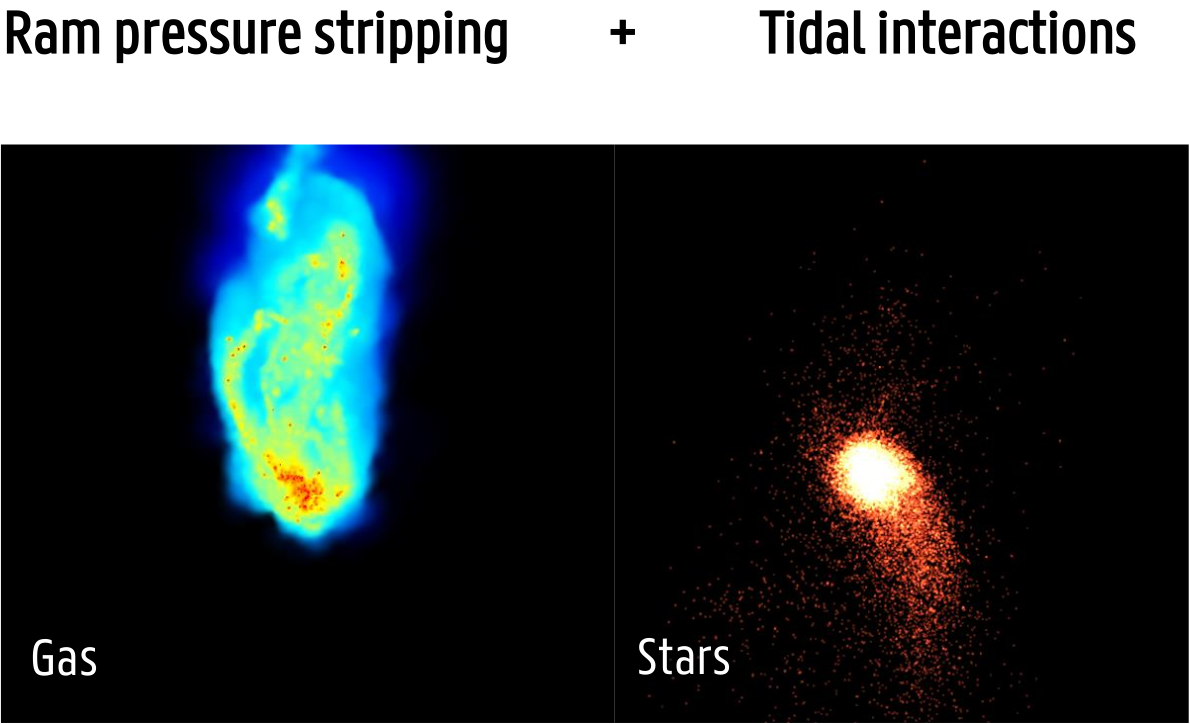
\includegraphics[width=\textwidth]{Gas_Tails}
  \caption{On the left the gaseous component of a simulated dwarf galaxy, color coded with projected density.
    On the right the stellar particles of the same galaxy.
   Different physical processes (of ram pressure stripping and tidal interactions) affecting the galaxy can lead to the creation of the curious effect of gaseous and stellar tails oriented in almost opposite directions.}
  \label{fig:tails}
\end{figure}


\section{This work}
To the best of our knowledge our work is the first to apply the Moving Box technique (see Section~\ref{sec:MovingBox}) to a galaxy cluster setup, using high definition simulations.
In comparison to earlier works our simulations take into account gas-rich realistic late-type galaxies.
To our knowledge none of them include such a high definition simulation starting from realistic late-type dwarf models.
In Chapter~\ref{ch:simulations} we introduce the techniques used for this kind of simulations and in Chapter~\ref{ch:sim_results} we present the main results.
%While I was able to build on the efforts of my predecessors, I have run and analyzed the simulations myself

In Chapter~\ref{ch:ngc1427a} \citep{Mastropietro2021} we take advantage of our simulation setup to propose a formation scenario for the galaxy NGC~1427A in the Fornax Cluster, including some falsifiable predictions.
Chapter~\ref{ch:manifolds} \citep{Canducci2021} we show the fruits of the collaboration with the Birmingham node within the SUNDIAL Innovative Training Network which has lead to the formulation of new techniques usable by astronomers to study low-dimensional manifolds in simulated ``jellyfish galaxies".
%Jellyfish galaxies is an interesting active research field whic
Chapter~\ref{ch:conclusions} gives an overview of the work and briefly present some ongoing research efforts.


